\begin{problem}[问题6.4]已知沿地面有一均匀来流, 流经
\vspace{-2em}
\begin{multicols}{2}
~

半径为$R$的半圆柱形暖棚, 求其所受到的
拔力.(设流动为理想不可压缩无旋流动, 暖棚内气压与无穷远处相等)

\begin{center}
\definecolor{cff0000}{RGB}{255,0,0}
\definecolor{cdb0024}{RGB}{219,0,36}
\definecolor{cb70049}{RGB}{183,0,73}
\definecolor{c92006d}{RGB}{146,0,109}
\definecolor{c6d0092}{RGB}{109,0,146}
\definecolor{c4900b7}{RGB}{73,0,183}
\definecolor{c2400db}{RGB}{36,0,219}
\definecolor{cd20000}{RGB}{210,0,0}
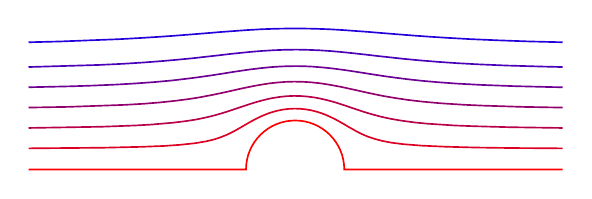
\begin{tikzpicture}[y=0.80pt, x=0.8pt,scale=0.75]
            \begin{scope}[cm={{4.55209,0.0,0.0,1.23779,(201.25,226.12)}}]
              \begin{scope}[xscale=0.125,yscale=0.459]
                      \begin{scope}[shift={(5.7805,24.704)}]
                        \path[draw=cdb0024,smooth,semithick]  (0.0000,0.0000)--
                           (79.1710,0.6840)-- 
                          (118.6300,1.5880) --
                           (143.1000,2.5410) --
                           (159.6800,3.6890) --
                          (175.9790,5.3990) --
                           (187.6600,7.3780) --
                           (196.0700,9.3570) --
                          (202.3690,11.3600) --
                          (209.1990,14.0710) --
                         (214.8090,16.7340) --
                          (219.6800,19.3480) --
                          (224.1690,21.9130) --
                          (228.7290,24.5760) --
                           (234.2900,27.8000) --
                         (238.1490,29.9010) --
                           (243.8800,32.8570) --
                          (247.7290,34.6160) --
                          (253.5400,36.9360) --
                          (257.3890,38.2560) --
                           (263.2900,39.8920) --
                           (269.1990,41.0890) --
                          (275.2190,41.8220) --
                         (281.2400,42.1150) --
                         (287.2700,41.9930) --
                          (293.2700,41.3580) --
                          (299.2400,40.3570) --
                          (305.1490,38.8170) --
                          (308.9990,37.6200) --
                          (314.8500,35.4220) --
                           (320.2400,32.9790) --
                           (324.4600,30.9270) --
                           (328.8800,28.4840) --
                           (334.1690,25.5280) --
                          (338.1990,23.0850) --
                          (342.5090,20.6670) --
                           (347.1000,18.0530) --
                         (352.3390,15.3660) --
                          (358.5090,12.7030) --
                          (366.2400,10.0410) --
                           (374.5400,7.8910) --
                           (383.8990,6.0590) --
                          (396.7290,4.4220) --
                          (416.1000,2.8830) --
                           (440.7290,1.7590) --
                          (472.0700,0.9040) --
                          (512.2900,0.3420) --
                          (563.8990,0.0000) --
                          (565.3200,0.0000);
                      \end{scope}
                      \begin{scope}[shift={(5.7805,46.324)}]
                        \path[draw=cb70049,smooth,semithick] 
                         (0.0000,0.0000) --
                         (77.1710,1.2940)-- 
                          (113.6800,2.6620) --
                           (129.6300,3.5660) --
                          (152.8090,5.5690) --
                           (166.6600,7.2550) --
                           (177.1000,8.9160) --
                          (187.0490,10.9440) --
                         (196.2400,13.1670) --
                          (205.4900,15.8290) --
                           (214.1990,18.6140) --
                           (220.1990,20.6660) --
                          (225.9300,22.5960) --
                         (233.9990,25.2590) --
                          (239.1690,26.8960) --
                          (246.7790,29.0450) --
                           (254.2190,30.8780) --
                          (259.1000,31.8300) --
                           (266.4190,32.9780) --
                           (273.7590,33.7110) --
                           (281.0200,34.0040) --
                          (288.3390,33.8330) --
                          (295.6090,33.2470) --
                           (302.9300,32.2940) --
                           (309.5890,30.9750) --
                          (315.2400,29.6810) --
                          (322.7590,27.7020) --
                           (327.8500,26.1140) --
                           (335.8090,23.5000) --
                          (341.3690,21.6190) --
                          (349.4900,18.8340) --
                          (356.8800,16.4650) --
                           (364.2400,14.2900) --
                          (372.6600,12.0430) --
                          (382.7100,9.8200) --
                           (395.1990,7.6700) --
                          (409.1690,5.7890) --
                          (422.1190,4.5430) --
                           (450.5090,2.6620) --
                           (470.4900,1.8810) --
                          ( (509.0490,0.8060) --
                           (561.3390,0.0490) --
                          (565.3200,0.0000);
                      \end{scope}
                      \begin{scope}[shift={(5.7805,67.943)}]
                        \path[draw=c92006d,smooth,semithick] (0.0000,0.0000) --
                         (41.9020,0.7330) -- 
                          (102.6090,2.9070) --
                           (121.7590,4.0310) --
                          (138.6090,5.3990) --
                         (155.7100,7.2070) --
                          (169.5590,9.0140) --
                           (181.4190,10.8950) --
                          (194.8290,13.4600) --
                         (204.3200,15.4390) --
                           (212.0700,17.1490) --
                         (222.8090,19.5920) --
                           (229.5090,21.0580) --
                         (239.1690,22.9870) --
                           (245.3690,24.1110) --
                          (254.3890,25.5520) --
                          (263.2900,26.5540) --
                          (272.0490,27.2380) --
                         (280.7790,27.4820) --
                          (289.5400,27.3600) --
                          (298.2700,26.8470) --
                          (307.1490,25.9430) --
                          (316.1000,24.6240) --
                          (322.2400,23.5490) --
                          (331.7290,21.7420) --
                          (340.5090,19.8120) --
                          (348.7100,18.0040) --
                         (356.1990,16.2940) --
                          (368.6300,13.6310) --
                          (378.1000,11.7990) --
                           (388.8990,9.9910) --
                           (401.5090,8.1100) --
                           (416.8290,6.3030) --
                           (436.1990,4.5440) --
                           (460.9490,2.9560) --
                           (481.1690,2.0520) --
                          (522.5590,0.7330) --
                           (557.1490,0.1220) --
                          (565.3200,0.0000);
                      \end{scope}
                      \begin{scope}[shift={(5.7805,89.465)}]
                        \path[draw=c6d0092,smooth,semithick] (0.0000,0.0000)  -- (42.5360,0.9520) -- (50.1950,1.1720) -- (68.6580,1.8070)--
                          (92.3410,2.8330) --
                           (113.8500,4.0790) --
                           (133.7290,5.5450) --
                          (152.3390,7.2550) --
                           (169.9990,9.3560) --
                         (181.7100,10.8950) --
                         (192.2190,12.4050) --
                         (206.2900,14.5850) --
                         (214.9300,16.0050) --
                       (227.0200,17.8050) --
                          (234.6300,18.8850) --
                           (245.7100,20.2550) --
                          (256.3690,21.3250) --
                         (265.9790,21.9650) --
                          (273.6800,22.3050) --
                           (283.9790,22.4050) --
                           (294.2400,22.1850) --
                          (301.1690,21.8350) --
                          (311.6800,20.9850) --
                           (322.4190,19.8650) --
                          (333.5890,18.3750) --
                           (341.4390,17.2450) --
                          (353.8090,15.3150) --
                           (362.6600,13.8950) --
                          (376.4190,11.7950) --
                         (388.4390,10.1380) --
                          (400.8800,8.5500) --
                           (415.2400,6.9620) --
                           (432.2190,5.4470) --
                           (452.9990,3.9080) --
                          (479.3390,2.4910) --
                           (514.3200,1.1720) --
                          (551.0700,0.2680) --
                          (563.4900,0.0000) -- (565.3200,0.0000);
                      \end{scope}
                      \begin{scope}[shift={(5.7805,110.91)}]
                        \path[draw=c4900b7,smooth,semithick] 
                           (0.0000,0.0000)  --
                           (74.1710,2.2000)
                           -- (100.3890,3.4500) --
                           (121.8090,4.8200) --
                          (139.8090,6.1800) --
                         (155.2900,7.5500) --
                           (173.0700,9.2400) --
                          (187.0490,10.8200) --
                         (197.8800,12.0200) --
                          (212.8290,13.7800) --
                          (223.7290,14.9300) --
                          (235.3690,16.1000) --
                          (248.0200,17.1300) --
                         (260.2900,17.8600) --
                          (272.2700,18.3200) --
                           (284.2400,18.4500) --
                           (296.1690,18.2000) --
                          (308.2700,17.7100) --
                          (320.6600,16.8600) --
                           (333.4900,15.7100) --
                        (342.3890,14.7600) --
                          (356.4900,13.2200) --
                           (368.0490,11.8500) --
                          (383.1690,10.2100) --
                          (395.4900,8.8500) --
                         (413.7100,7.0900) --
                           (433.2900,5.5000) --
                          (452.8800,4.1300) --
                          (476.5090,2.8400) --
                           (505.9300,1.5900) --
                          (543.0490,0.5200) --
                         (565.3200,0.0000);
                      \end{scope}
                      \begin{scope}[shift={(5.7805,137.17)}]
                        \path[draw=c2400db,smooth,semithick] (0.0000,0.0000) -- 
                          (34.1950,0.8600)-- (96.5400,3.3000) --
                           (119.7100,4.6000) --
                           (137.7590,5.7400) --
                           (153.8290,6.8700) --
                            (175.0700,8.5300) --
                            (187.7790,9.5600) --
                           (205.3200,11.0200) --
                           (216.4600,11.8300) --
                            (231.8500,12.9500) --
                            (246.7290,13.8100) --
                            (261.1000,14.3200) --
                           (275.2190,14.5900) --
                            (289.2400,14.5900) --
                           (303.3890,14.3200) --
                            (317.7590,13.8100) --
                            (332.6300,12.9500) --
                           (348.0200,11.8300) --
                            (359.1490,11.0200) --
                           (376.6800,9.5600) --
                           (389.4600,8.5300) --
                           (410.6300,6.8700) --
                           (426.7100,5.7400) --
                           (444.7790,4.6000) --
                         (467.9300,3.3000) --
                           (497.9790,2.0100) --
                           (530.2900,0.8600) --
                           (565.3200,0.0000);
                      \end{scope}
                      \begin{scope}[shift={(235.98,-2.7534)}]
                      \draw[red,semithick](-230,5)--(0,5) arc(-180:-360:52)--(335,5);
                      \end{scope}
              \end{scope}
\end{scope}
\end{tikzpicture}

\end{center}
\end{multicols}
\end{problem}

\begin{solution}
\textbf{解:} 该问题可看作无环量圆住绕流问题的上半平面, 故其复速度势为
\[
W(z) = v_\infty\big(z+\frac{R^2}{z}\big)
\]
对应的势函数和流函数分别为
\[
\varphi = v_\infty\big(r+\frac{R^2}{r}\big)\cos\theta,{~~~} \psi = v_\infty\big(r+\frac{R^2}{r}\big)\sin\theta
\]
因此速度在$r$和$\theta$上的速度分量分别为
\[
v_r = \frac{\partial\varphi}{\partial r} = v_\infty\big(1-\frac{R^2}{r^2}\big)\cos\theta,{~~~}
v_\theta = \frac{1}{r}\frac{\partial\varphi}{\partial\theta} = -v_\infty\big(1+\frac{R^2}{r^2}\big)\sin\theta
\]
半圆柱形暖棚表面有$v_r=0$, $v_\theta=-2v_\infty\sin\theta$, 因此对半圆柱形暖棚表面和无穷远处
应用伯努力方程
\[
\frac{v_\infty^2}{2} + \frac{p_\infty}{\rho} = \frac{v_\theta^2}{2} + \frac{p_\theta}{\rho}
{~~}\Longrightarrow{~~} p_\theta = p_\infty + \frac{\rho}{2}v_\infty^2(1-4\sin^2\theta)
\]
因此拔力为
\begin{eqnarray}
F_Y &=& \int_0^\pi (p_\infty - p_\theta)\cdot R\sin\theta d\theta\nonumber\\
&=& \frac{1}{2} \rho Rv_\infty^2\int_0^\pi (4\sin^2\theta-1)\sin\theta d\theta\nonumber\\
&=& \frac{1}{2} \rho Rv_\infty^2\int_0^\pi (4\cos^2\theta-3)d(\cos\theta)\nonumber\\
&=& \frac{1}{2} \rho Rv_\infty^2\Big[
\frac{4}{3}\cos^3\theta-3\cos\theta
\Big]_0^\pi\nonumber\\
&=& \frac{5}{3}\rho Rv_\infty^2\nonumber
\end{eqnarray}
\end{solution}
